\section{提案手法} \label{sec4}
本章では，五つのコンポーネントから構成される提案手法の概要ついて述べる．提案手法は，LLMとシミュレータから取得した家庭環境知識を用いて，タスクを実行するためのアクションを逐次的に生成する．さらに，LLMを用いて生成されたアクションが前提条件を満たしているかを検証する．前提条件を満たしていない場合は，現在の環境状況に基づいて代替アクションを再生成する．提案手法の構成図を~\ref{proposed_method}に示す．

\begin{figure}[t]
  \begin{center}
    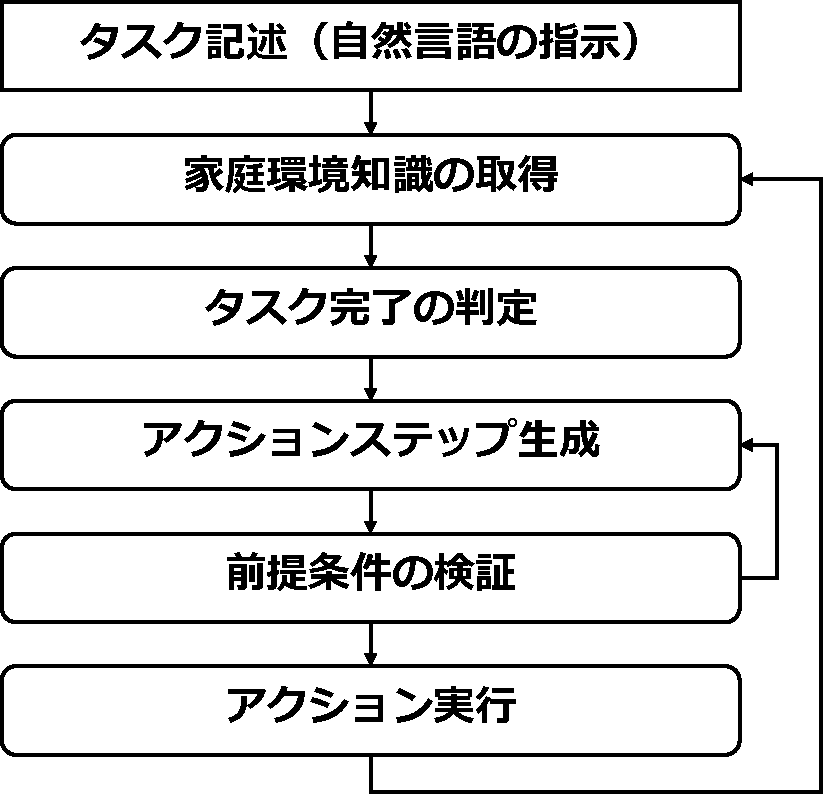
\includegraphics[width=8cm]{figures/proposed_method.pdf}
    \caption{提案手法の構成}
    \label{proposed_method}
  \end{center}
\end{figure}


\subsection{家庭環境知識の取得} \label{sec4.1}
\ref{proposed_method}の「家庭環境知識の取得」では，シミュレータから家庭環境知識を取得し，自然言語で記述する．ただし，この知識は，エージェントとタスクの記述に含まれる物体に関する知識に限定される．

エージェントに関する知識には，エージェントの状態，物体や部屋との関係，および関係を持つ物体の状態が含まれる．
物体に関する知識には，物体の状態，他の物体や部屋との関係，および関係を持つ他の物体の状態が含まれる．


\subsection{タスク完了の判定} \label{sec4.2}
\begin{figure*}[tb]
    \begin{lstlisting}[caption=「タスク完了の判定」で用いるプロンプトテンプレート, label=prompt1]
The current states in the home are as follows: 
@\textcolor{red}{\textit{[ Home environment knowledge ]}}@

If the following task has already completed based on the current states, output "End"; otherwise, output "Continue."
Task: @\textcolor{red}{\textit{[ Task description ]}}@
    \end{lstlisting}
\end{figure*}

\begin{figure*}[tb]
    \begin{lstlisting}[caption=「アクションステップ生成」で用いるプロンプトテンプレート, label=prompt2]
You need to generate a next action step for completing a household task.

Allowed actions: @\textcolor{red}{\textit{[ Allowed actions ]}}@
Output format: @\textcolor{red}{\textit{[ Output format ]}}@

Example Task: @\textcolor{red}{\textit{[ An example Task ]}}@
@\textcolor{red}{\textit{[ Action plan for the example task ]}}@

The current states in the home are as follows: 
@\textcolor{red}{\textit{[ Home environment knowledge ]}}@

Generate an only next action step to complete the following task and output only that.
Task: @\textcolor{red}{\textit{[ Task description ]}}@
Step1:
    \end{lstlisting}
\end{figure*}

\ref{proposed_method}の「タスク完了の判定」では，LLMが家庭環境知識に基づき，タスクが完了しているかを判定する．

本コンポーネントで用いるプロンプトテンプレートをListing~\ref{prompt1}に示す．本プロンプトテンプレートは，
家庭環境知識（Listing~\ref{prompt1}の2行目）とタスク記述（Listing~\ref{prompt1}の5行目）の二つの要素から構成される．ここで，LLMの出力が``End''であれば処理を終了し，``Continue''であれば次のプロセスへ移行する．

さらに，最大試行回数を設定して，タスク終了の判定を行う．これは，無限ループを回避するために導入した処理であり，設定した試行回数を達した場合に全体のループ処理を終了する．試行回数は0から開始し，このコンポーネントを通過するたびに1加算される．試行回数の上限の決定方法は，第~\ref{sec5.2}で述べる．


%\subsection{試行回数によるタスク終了判定} \label{sec4.3}
%\ref{proposed_method}の「試行回数によるタスク終了判定」では，設定した試行回数を達した場合に処理を終了する．これは，無限ループを回避するために導入している．試行回数は0から開始し，このコンポーネントを通過するたびに1加算される．
%試行回数の上限の決定方法は，第~\ref{sec5.2}で述べる．

\subsection{アクションステップ生成} \label{sec4.3}

\ref{proposed_method}の「アクションステップ生成」では，LLMと家庭環境知識を用いて，タスクを達成するために必要な次のアクションステップを一つ生成する．

本コンポーネントで用いるプロンプトテンプレートをListing~\ref{prompt2}に示す．本プロンプトテンプレートは，「実行可能なアクションとその出力形式（Listing~\ref{prompt2}の3行目と4行目）」，「One-shot学習用の例（タスクと行動計画）（Listing~\ref{prompt2}の6行目と7行目）」，「家庭環境知識（Listing~\ref{prompt2}の10行目）」，「タスクとアクションの実行履歴（Listing~\ref{prompt2}の13，14行目）」の四つの要素から構成される．



\subsection{前提条件の検証} \label{sec4.4}
\begin{figure*}[tb]
  \begin{center}
    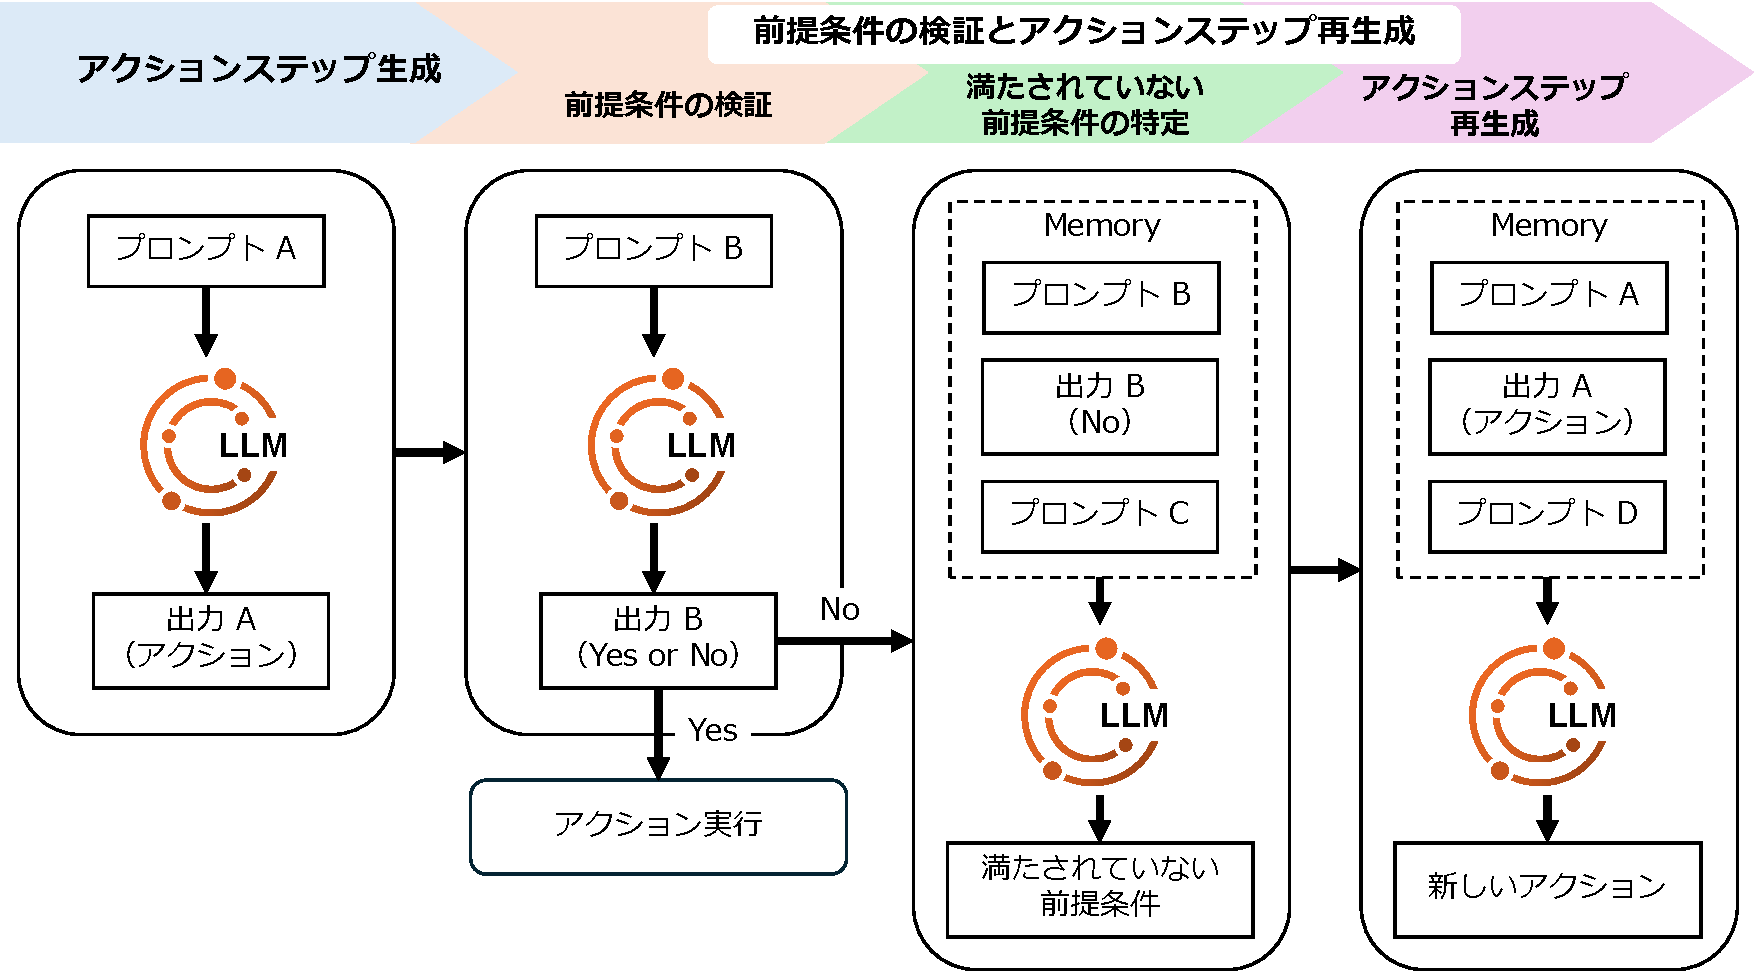
\includegraphics[width=\textwidth]{figures/Precheck.pdf}
    \caption{前提条件の検証とアクションステップ再生成の概要}
    \label{Precheck}
  \end{center}
\end{figure*}

\begin{figure*}[tb]
    \begin{lstlisting}[caption=\ref{Precheck}の「前提条件の検証」における「プロンプトB」の生成に用いるプロンプトテンプレート, label=prompt3]
The current states in the home are as follows: 
@\textcolor{red}{\textit{[ Home environment knowledge ]}}@

If the current states satisfies the preconditions, output "Yes"; otherwise, output "No."
Preconditions: @\textcolor{red}{\textit{[ Preconditions ]}}@
    \end{lstlisting}
\end{figure*}

\begin{figure*}[tb]
    \begin{lstlisting}[caption={\ref{Precheck}の「満たされていない前提条件の特定」における「プロンプトC」の生成に用いるプロンプトテンプレート}, label=prompt4]
Which the preconditions are not met satisfied? Output only that.
Preconditions: @\textcolor{red}{\textit{[ Preconditions ]}}@
    \end{lstlisting}
\end{figure*}

\ref{proposed_method}の「前提条件の検証」では，LLMを用いて，生成されたアクションステップを実行するための前提条件を，現在の状況が満たしているかどうかを検証する．さらに，前提条件を満たしていなかった場合には，満たされていない前提条件を特定し，それに基づいてアクションステップの再生成を行う．一連のプロセスの概要を~\ref{Precheck}に示す．

初めに，Listing~\ref{prompt3}に示すプロンプトテンプレートを用いて，前提条件の検証を行う．本プロンプトテンプレートは，家庭環境知識（Listing~\ref{prompt3}の2行目）とアクションの前提条件（Listing~\ref{prompt3}の5行目）の二つの要素から構成される．前提条件の記述は事前に準備しておき，生成されたアクションに応じて適切な前提条件を選択する．LLMの出力が``Yes''である場合は，「アクション実行」に移る．LLMの出力が``No''である場合は，Listing~\ref{prompt4}に示すプロンプトテンプレートを用いて，満たされていない前提条件を特定する．ここでは，前提条件の検証で用いたプロンプトとその出力（\ref{Precheck}のプロンプトBと出力B）を対話履歴としてLLMに与える．

満たされていない前提条件の特定後は，Listing~\ref{prompt5}に示すプロンプトテンプレートを用いて，アクションステップの再生成を行う．本プロンプトテンプレートは，「生成されたアクション（Listing~\ref{prompt5}の1行目）」，「特定された満たされていない前提条件（Listing~\ref{prompt5}の2行目）」，「タスクとアクションの実行履歴（Listing~\ref{prompt5}の5，6行目）」の三つの要素から構成される．また，「アクションステップ生成」で用いたプロンプトとその出力（\ref{Precheck}のプロンプトAと出力A）を，対話履歴としてLLMに与える．

%\capwidth=\linewidth
%\lstinputlisting[caption={「満たされていない前提条件の特定」で用いるプロンプトテンプレート（~\ref{precheck}のプロンプトC）},float=tb,label=prompt4-2]{"./listings/Listing4.txt"}


\begin{figure*}[tb]
    \begin{lstlisting}[caption=\ref{Precheck}の「アクションステップ再生成」における「プロンプトD」の生成に用いるプロンプトテンプレート, label=prompt5]
@\textcolor{red}{\textit{[ Generated action step ]}}@ can not execute, because it is not satisfied the following 
precondition: @\textcolor{red}{\textit{[ Preconditions ]}}@

Regenerate an only next action step to complete the following task and output only that.
Task: @\textcolor{red}{\textit{[ Task description ]}}@
@\textcolor{red}{\textit{[ Action execution history ]}}@
Step n: 
    \end{lstlisting}
\end{figure*}

\subsection{アクション実行} \label{sec4.5}
\ref{proposed_method}の「アクション実行」では，生成したアクションステップをシミュレータ上で実行する．また，実行に成功した場合には，実行したアクションステップを実行履歴として\ref{proposed_method}の「アクションステップ生成」で用いるプロンプトの末尾に追加する．その後「家庭環境知識の取得」を再度行い，処理が終了するまで一連のプロセスを繰り返す．なお，アクションの実行に失敗した場合も処理を終了する．


\subsection{実装} \label{sec4.6}
本節では，提案手法の実装について述べる．
提案手法の実装で用いるシミュレータに必要な機能条件を以下に示す．

\begin{itemize}
    \item シミュレータの内部データとして，完全な家庭環境知識を取得することが可能であり，それには物体の状態や物体間の関係，エージェントと物体間の関係が表現されている．
    \item 前進や回転，アームを動かすなどの細かい動作でエージェントを動作させるのではなく，対象物とその識別番号を指定することで移動やインタラクションが可能な高レベルのコマンドが用意されている．
    \item アクションを実行するための前提条件が定義されている．
\end{itemize}

本研究では，これらの条件を満たすシミュレータとしてVirtualHome (VH)~\cite{Puig_2018_CVPR}のバージョン2.3を用いて提案手法を実装した．
VHは，高レベルのコマンドが提供されているのが特徴的である．一方，他のシミュレータでは，細かい動作でエージェントを動かすことが多い．
また，VHの家屋は，4から5の複数の部屋で構成されており，多くの部屋や物体が存在する環境下で，実験を行うことが可能である．

VHは，仮想家庭内で活動をシミュレートすることを目的としたシミュレータである．VHの環境は，JSON形式のグラフ構造として表されている．環境内に存在するオブジェクトのリストを``nodes''キーの値として記述し，部屋や物，またそれらに関する識別番号，位置座標，物の状態といったセマンティックデータを定義している．また，``nodes''キーの値として記述された各オブジェクトの識別番号を指定し，二つのオブジェクトの関係のリストを``edges''キーの値として定義している，

VHでは，一連のアクションステップを記述したアクションスクリプトに基づいて，エージェントを行動させることができる．各ステップは，エージェントが実行するアクション，対象となるオブジェクト，およびそのオブジェクトの識別番号（ID）で構成される（例：[WALK] $\langle livingroom \rangle$ (336)）．各アクションには，実行される環境の制約を示す前提条件が定められており，アクションを実行する際には，その前提条件を満たしている必要がある．VHのDocumentation\footnote{\url{http://virtual-home.org/documentation/master/kb/actions.html}}やGitHub\footnote{\url{https://github.com/xavierpuigf/virtualhome/tree/master/virtualhome/simulation}}に，各アクションの満たすべきすべての前提条件が記載されている．